\section{Problem 3}
\begin{frame}
        \frametitle{Problem 3(a) – Linear Fitting}

        \begin{equation}
            \begin{bmatrix}
                x_1 & 1 \\
                x_2 & 1 \\
                \vdots & \vdots \\
                x_n & 1
            \end{bmatrix}
            \begin{bmatrix}
                a_1 \\ a_0
            \end{bmatrix}
            =
            \begin{bmatrix}
                y_1 \\ y_2 \\ \vdots \\ y_n
            \end{bmatrix}
        \end{equation}
        \begin{equation}
            d\left(b,C\left(A\right)\right) = \left||Ax-b|\right|
        \end{equation}

    \end{frame}

\begin{frame}[fragile] 
    \frametitle{Problem 3(a) – Codes}
    % 代码块参数:语言,标题
    % 请减少代码初始的缩进
    \begin{codeblock}{c++}{C++ Codes}
        //ATAx = ATb
        F_result = (A.transpose() * A).ldlt().solve(A.transpose() * b);
        cout << "The solution using normal equations is:\n"
            << F_result << endl;
        cout << "The distance is : " << (A * F_result - b).norm() << endl;
    \end{codeblock}
    % \begin{figure}
    %     \centering
    %     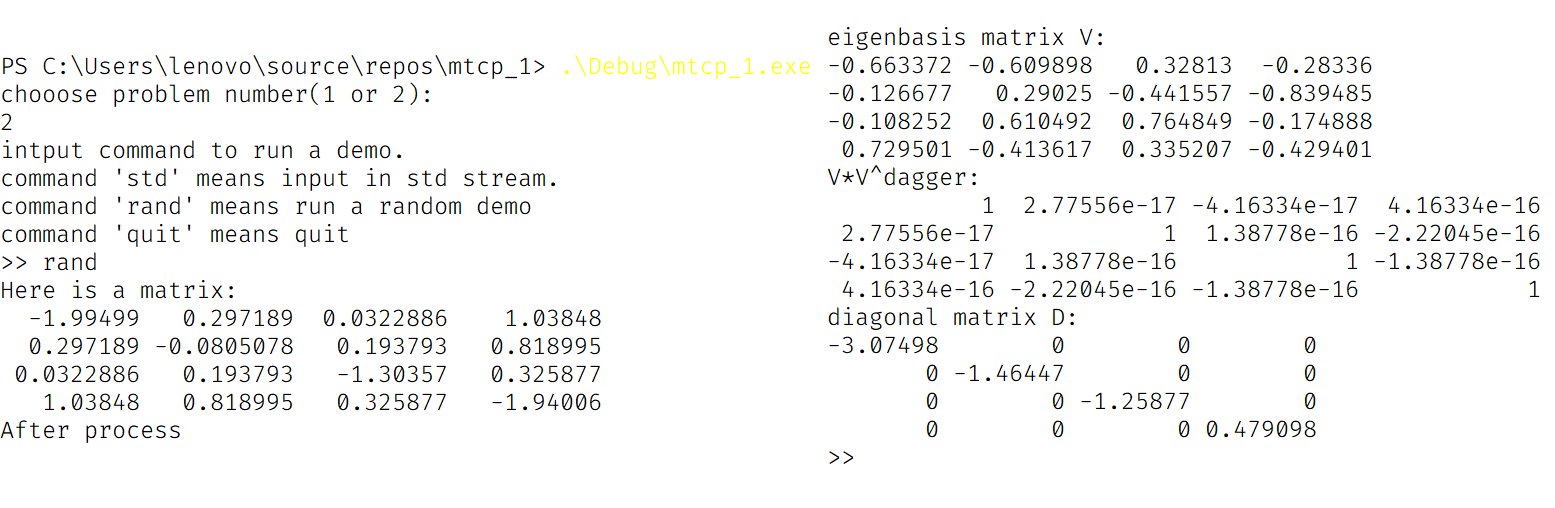
\includegraphics[height = 0.8\textheight]{img/result2.png}
    % \end{figure}
\end{frame}

\begin{frame}         % 注意添加 fragile 标记
    \frametitle{Problem 3(a) – Program Results}

    \begin{figure}
        \centering
        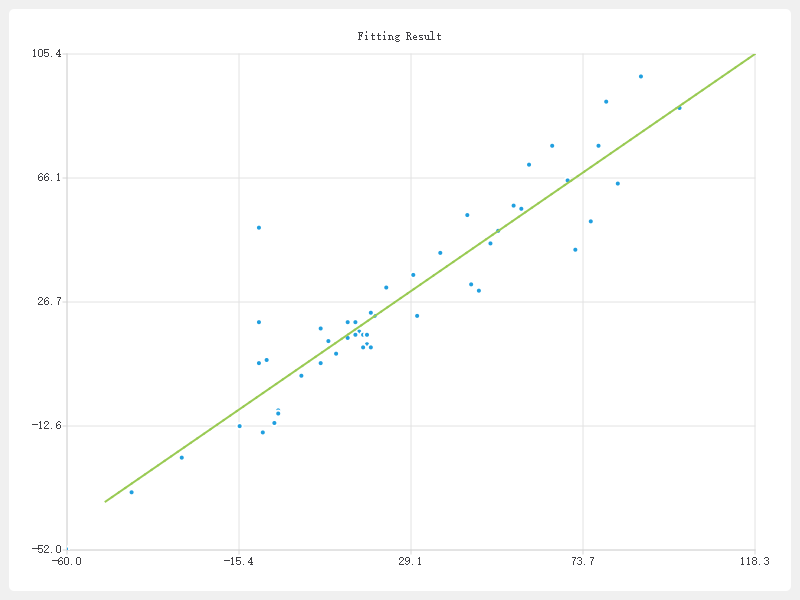
\includegraphics[height = 0.5\textheight]{img/result3_1.png}
    \end{figure}
        \begin{equation}
        d(b,C(A))=84.89
    \end{equation}
\end{frame}
\begin{frame}
        \frametitle{Problem 3(b) – Parabolic Fitting}

    % \begin{figure}
    %     \centering
    %     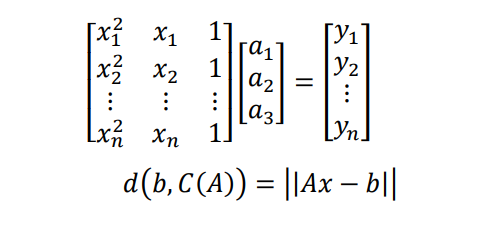
\includegraphics[height = 0.5\textheight]{img/setup3_2.png}
    % \end{figure}
    \begin{equation}
        \begin{bmatrix}
            x_1^2 & x_1 & 1 \\
            x_2^2 & x_2 & 1 \\
            \vdots & \vdots & \vdots \\
            x_n^2 & x_n & 1
        \end{bmatrix}
        \begin{bmatrix}
            a_2 \\ a_1 \\ a_0
        \end{bmatrix}
        =
        \begin{bmatrix}
            y_1 \\ y_2 \\ \vdots \\ y_n
        \end{bmatrix}
    \end{equation}
    \begin{equation}
        d\left(b,C\left(A\right)\right) = \left||Ax-b|\right|
    \end{equation}

    \end{frame}
\begin{frame}[fragile] 
    \frametitle{Problem 3(b) – Codes}
    % 代码块参数:语言,标题
    % 请减少代码初始的缩进
    \begin{codeblock}{c++}{C++ Codes}
        for (int i = 0; i < N; i++) 
        {
            A(i, 0) = mat(i, 0) * mat(i, 0);
            A(i, 1) = mat(i, 0);
            A(i, 1) = 1;
            b(i) = mat(i, 1);
        }
        //ATAx = ATb
        F_result = (A.transpose() * A).ldlt().solve(A.transpose() * b);
        cout << "The distance is : " << (A * F_result - b).norm() << endl;
    \end{codeblock}
    % \begin{figure}
    %     \centering
    %     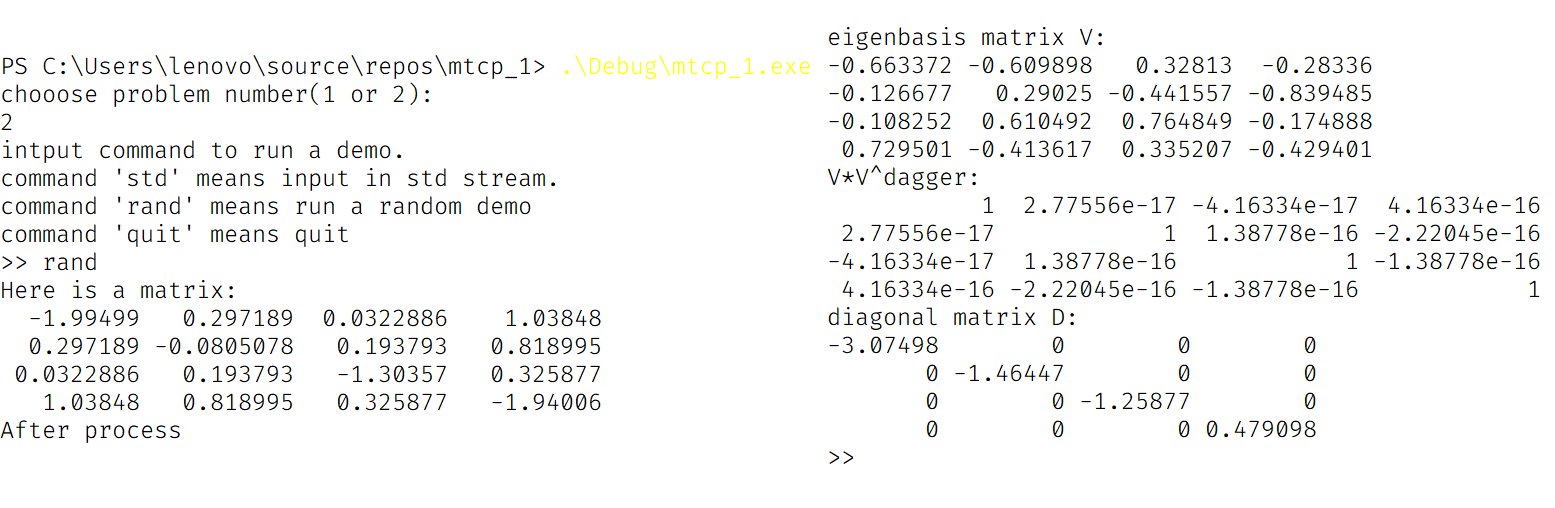
\includegraphics[height = 0.8\textheight]{img/result2.png}
    % \end{figure}
\end{frame}

\begin{frame}         % 注意添加 fragile 标记
    \frametitle{Problem 3(b) – Program Results}

    \begin{figure}
        \centering
        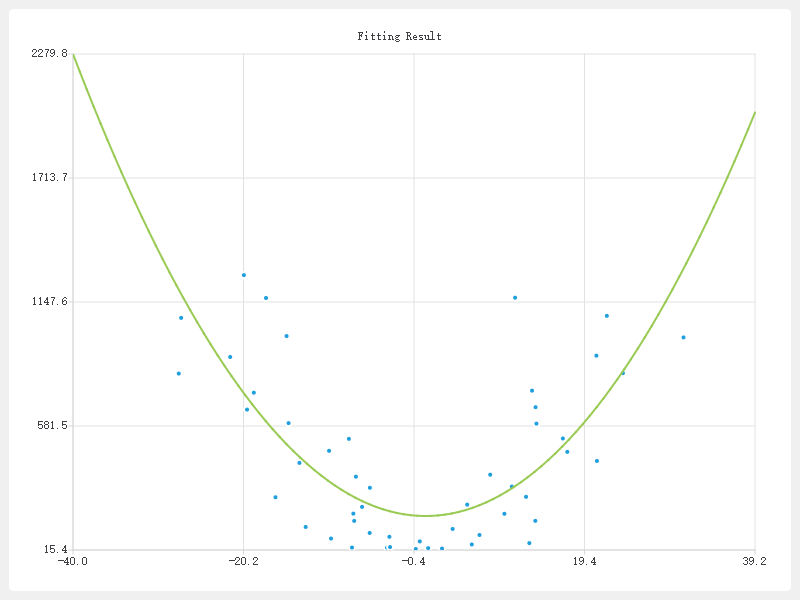
\includegraphics[height = 0.5\textheight]{img/result3_2.png}
    \end{figure}
        \begin{equation}
        d(b,C(A))=1789.58
    \end{equation}
\end{frame}
